
\documentclass[a0paper,portrait]{baposter}

\usepackage{relsize}
\usepackage{bbding}
\usepackage{pifont}

\usepackage[utf8]{inputenc} %unicode support
\usepackage[T1]{fontenc}
\usepackage{amsmath,amssymb,graphicx}
\usepackage[spanish, es-tabla]{babel}    \spanishdecimal{.}
\usepackage{float}
\usepackage{physics}
\usepackage{pifont}

\usepackage[dvipsnames]{xcolor}
\usepackage{setspace}
\usepackage{mwe} % new package from Martin scharrer
\usepackage{tikz,pgfplots}
\usepackage[fontsize=10pt]{\fontfamily{qcr}}


\usepackage[font=tiny,labelfont=bf]{caption}
\usepackage[theorems,skins]{tcolorbox}


\usepackage{xcolor}
\definecolor{bluemath}{rgb}{0, 1, 0}
\definecolor{blueUNAM}{RGB}{0,60,113}
\definecolor{orangemath}{rgb}{1, .5, .5}
\definecolor{lblue}{RGB}{134,165,169}
\definecolor{bluenice}{RGB}{23,176,199}
\definecolor{gris}{RGB}{118,118,118}
\definecolor{botwgreen1}{RGB}{83,111,80}	
\definecolor{botwgreen2}{RGB}{146,197,130}	
\definecolor{mxpink}{RGB}{229,0,92}	
\definecolor{greenMathematica}{rgb}{0.560181, 0.691569, 0.194885}
%\selectcolormodel{cmyk}
\definecolor{darkgreen}{cmyk}{0.8,0,0.8,0.45}
\definecolor{lgreen}{cmyk}{0.8,0,0.8,0.25}

\graphicspath{{figures/}} % Directory in which figures are stoorange

\newcommand*\tick{\item[\color{orange}  \blacksquare ]}
\newcommand{\compresslist}{%
	\setlength{\itemsep}{0pt}%
	\setlength{\parskip}{1pt}%
	\setlength{\parsep}{0pt}%
}

\begin{document}
	\typeout{Poster rendering started}
	\background{ }
	\begin{poster}{
			columns = 4, 
			grid=false,
			headerborder=open, % Adds a border around the header of content boxes
			colspacing=.5em, % Column spacing
			bgColorOne=white, % Background color for the gradient on the left side of the poster
			bgColorTwo=white, % Background color for the gradient on the right side of the poster
			borderColor=white,%darkgreen, % Border color
			headerColorOne= blueUNAM, % Background color for the header in the content boxes (left side)
			headerColorTwo= bluenice, % Background color for the header in the content boxes (right side)
			headerFontColor=white,%white, % Text color for the header text in the content boxes
			%headershade= shade-tb, %plain
			boxColorOne=white, % Background color of the content boxes
			textborder=none, %rectangle, % Format of the border around content boxes, can be: none, bars, coils, triangles, rectangle, rounded, roundedsmall, roundedright or faded
			eyecatcher=true, % Set to false for ignoring the left logo in the title and move the title left
			headerheight=0.09\textheight, % Height of the header
			headershape=rectangle, % Specify the rounded corner in the content box headers, can be: rectangle, small-rounded, roundedright, roundedleft or rounded
			headerfont=\Large, % Large, bold and sans serif font in the headers of content boxes
			%textfont={\setlength{\parindent}{1.5em}}, % Uncomment for paragraph indentation
			linewidth=2pt % Width of the border lines around content boxes
		}
		%
		%----------------------------------------------------------------------------------------
		%	TITLE AND AUTHOR NAME
		%----------------------------------------------------------------------------------------
		%%
		{
\includegraphics[width=2.7cm]{logo_unam}
			
		} 
		{%Titulo
			\vspace{0.05em}\huge{\color{blueUNAM}{ %Sans Serif
					{\noindent 
						Localización espectral de resonancias plasmónicas en nanoesferas tipo Drude de tamaño arbitrario }}}
		}
		{%Autores
			\normalsize\vspace{0.5em}\\ 
			{\color{mxpink}\textbf{Luna González, Dana L.$^1$}}, Urrutia Anguiano, Jonathan A.$^2$  y Reyes Coronado, Alejandro$^3$
			\vspace{0.3em}\\
			\footnotesize{Departamento de Física, Facultad de Ciencias, Universidad Nacional 	Autónoma de México
				\vspace{0.2em}\\
				{\color{mxpink}\textbf{$^1$dana.larissalg@ciencias.unam.mx}}, $^2$jaurrutia.95@ciencias.unam.mx, $^3$coronado@ciencias.unam.mx}
		}
		{
\includegraphics[width=2.85cm]{logo_ciencias}
		} %the author(s)     
		\vspace*{-10cm} 
		\headerbox{ \textbf{ Resumen}}{name=abstract,column=0,row=0, span=4}{\scriptsize \begin{singlespace}
				La {\color{mxpink}\textbf{nanoplasmónica}} es el estudio de la respuesta electromagnética en sistemas con respuesta metálica a la nanoescala, es decir, con dimensiones menores a 100 nm. En sistemas espacialmente confinados a esta escala, se presenta el fenómeno de {\color{mxpink}\textbf{resonancia de plasmón de superficie localizado}}, resultado del acoplamiento entre los electrones libres de un metal con el campo electromagnético incidente que ilumina al sistema. Este fenómeno se puede emplear en aplicaciones como la espectroscopía y la medicina, debido a la sintonización de dichas resonancias a una frecuencia específica según las propiedades morfológicas del sistema. La teoría de Mie es una solución analítica a las ecuaciones de Maxwell que describe la excitación de la resonancia plasmónica de superficie para partículas metálicas esféricas iluminadas por una onda electromagnética plana mediante una suma de contribuciones multipolares de modos eléctricos y magnéticos, con los cuales puede calcularse la sección transversal de extinción, cuyo máximo corresponde a la excitación del plasmón de superficie localizado. En este trabajo, se estudia teórica y numéricamente la localización espectral de las resonancias plasmónicas excitadas en {\color{mxpink}\textbf{partículas esféricas}} caracterizadas por una función dieléctrica descrita por el {\color{mxpink}\textbf{modelo de Drude}} en función de su {\color{mxpink}\textbf{radio}}. Para determinar numéricamente la posición espectral de las resonancias plasmónicas de los primeros órdenes multipolares eléctricos y magnéticos, se calcula la sección transversal de extinción para cada uno de ellos, y se identifica la frecuencia que maximiza estas cantidades. Finalmente, se contrastan los resultados obtenidos con la condición de resonancia en el {\color{mxpink}\textbf{límite de partícula pequeña}} obtenida analíticamente. Con base en los resultados, se presentan curvas del corrimiento al rojo de las resonancias plasmónicas de superficie localizadas para partículas esféricas conforme el límite de partícula pequeña deja de ser válido.
			\end{singlespace}
			
		}
		%-------Resumen---------------------------
		%-------abstract---------------------------
		
		
		
		%-------Introducción---------------------------
		%-------intro---------------------------
		\headerbox{\textbf{1) Introducción}}{name=intro,column=0,below=abstract,span=2}{\footnotesize 
			La interacción luz-materia puede estudiarse clásicamente mediante la {\color{mxpink}\textbf{absorción}} y el {\color{mxpink}\textbf{esparcimiento}}, cuyo efecto combinado resulta en la {\color{mxpink}\textbf{extinción}} del haz incidente \cite{Bohren}. En los últimos años, se han estudiado las propiedades ópticas de partículas de diferentes formas y tamaños debido a sus potenciales aplicaciones en ciencia aplicada y nanotecnología \cite{Mendez}.
			
			
			\begin{minipage}[c]{.35\linewidth}
				\centering
				{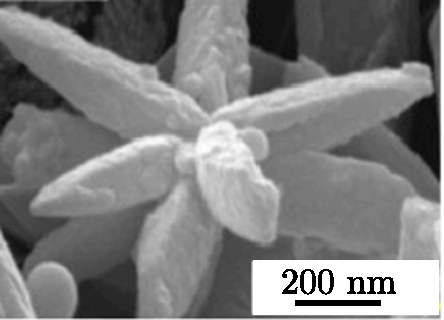
\includegraphics[width=4cm]{flower.pdf}}
				\begin{singlespace}
					\tiny Tomada y adaptada de \cite{Mendez}.
				\end{singlespace}
					
			\end{minipage}
			\begin{minipage}[c]{.65\linewidth}
				\centering
				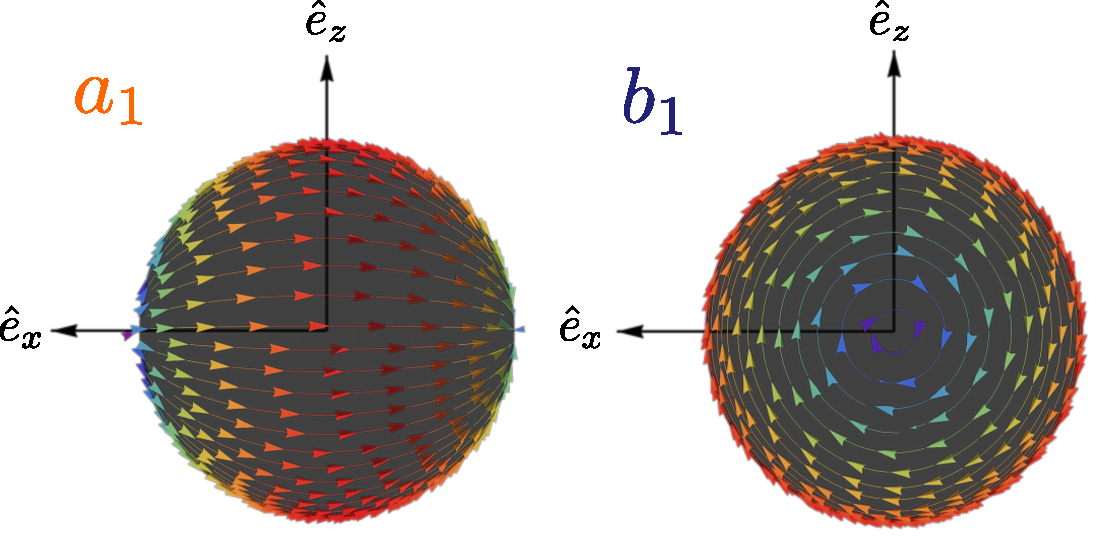
\includegraphics[width=6.5cm]{dipoleelectric.pdf}
			\end{minipage}	
		
			
		}
		
		
		\headerbox{ \textbf{2) Teoría de Mie}}{name=MieTh,column=0,below=intro,span=2}{\footnotesize 
			La solución al problema de absorción  y esparcimiento de luz por una {\color{mxpink}\textbf{partícula esférica}} se conoce como {\color{mxpink}\textbf{teoría de Mie}}. Esta es una solución analítica a las ecuaciones de Maxwell que, para partículas metálicas iluminadas por una onda electromagnética (EM) plana, describe la excitación de la {\color{mxpink}\textbf{resonancia plasmónica de superficie localizada}} (LSPR). Los campos EMs dentro de la partícula y los esparcidos por ésta se escriben como una combinación lineal de modos multipolares eléctricos y magnéticos modulados por los denominados {\color{mxpink}\textbf{coeficientes de Mie}}. En particular, los coeficientes correspondientes al campo esparcido están dados por \cite{Bohren}:\\
			\begin{minipage}[c]{.55\linewidth}
				{\footnotesize
					$$  \tcboxmath[colback=orange!15!white ,colframe=orange,size=title]{a_\ell=\frac{m\psi_{\ell}(mx)\psi_{\ell}'(x)-\psi_{\ell}(x)\psi_{\ell}'(mx)}{m\psi_{\ell}(mx)\xi_{\ell}'(x)-\xi_{\ell}(x)\psi_{\ell}'(mx)}, }$$ $$\tcboxmath[colback=bluenice!15!white ,colframe=blueUNAM, size=title]{b_{\ell}=\frac{\psi_{\ell}(mx)\psi_{\ell}'(x)-m\psi_{\ell}(x)\psi_{\ell}'(mx)}{\psi_{\ell}(mx)\xi_{\ell}'(x)-m\xi_{\ell}(x)\psi_{\ell}'(mx)}, }$$ 
					con $\psi_{\ell}(\rho)=\rho j_{\ell}(\rho)$ y $\xi_{\ell}(\rho)=\rho h_{\ell}^{(1)}(\rho)$ las funciones de Ricatti-Bessel, dadas en términos de las 	funciones esféricas de Bessel $j_{\ell}$ y las funciones}
			\end{minipage}
			\begin{minipage}[c]{.45\linewidth}
				%\centering
				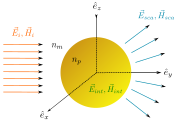
\includegraphics[width=5cm]{scattering.png}
			\end{minipage}	\\
		 funciones esféricas de Hankel de primer tipo $h_{\ell}^{(1)}$,  $m=n_p/n_m$  y $x=2 \pi n_m/a$ el parámetro de tamaño. La {\color{mxpink}\textbf{sección transversal de extinción}} se escribe en términos de los coeficientes de Mie como \cite{Bohren}:
			$$ \tcboxmath[colback=greenMathematica!15!white ,colframe=greenMathematica,size=title]{C_{ext}=\frac{2\pi}{k^2}\sum_{n=1}^{\infty}(2n+1)\:\text{Re}\{a_{\ell}+b_{\ell}\},}$$
			donde $\text{Re}\{\cdot\}$ representa la parte real de un número complejo.			
		}
		
		\vspace{-1mm}
		%-------CSM---------------------------
		%-------csm---------------------------
		\headerbox{\textbf{3) Esferas plasmónicas en el límite $k_m a \ll 1$
		}}{name=mdd,column=0,below=MieTh,span=2}{\footnotesize 
			La respuesta electromagnética de un metal puede describirse mediante su índice de refracción dado en términos del  {\color{mxpink}\textbf{modelo de Drude}}, que representa la solución de la ecuación de movimiento de los electrones libres de un material en presencia de un campo eléctrico oscilante  \cite{Novotny}, el cual está dado por: 
			
			\begin{minipage}[c]{0.55\textwidth}
				$$\text{(1)}\hspace{1cm} \tcboxmath[colback=greenMathematica!15!white ,colframe=greenMathematica,size=title]{n_p =\sqrt{1-\frac{\omega_p^2}{\omega(\omega+i\gamma)}},}$$
			\end{minipage}
				\begin{minipage}[c]{0.45\textwidth}
				donde $\omega_p$ es la frecuencia de plasma y $\gamma$ la constante fenomenológica de amortiguamiento, ambos parámetros propios de cada material.
			\end{minipage}			
			
			
			\vspace{0.2cm}
			Considerando el límite de partícula pequeña, la expansión de las funciones de Ricatti-Bessel \cite{Abramowitz} y $n_m=1$, al minimizar el denominador de los coeficientes de Mie, se puede obtener una relación sencilla para las condiciones de resonancia:\\
			
		
			\begin{minipage}[c]{.55\linewidth}
				\centerline{ {\color{orange}\textbf{Multipolos eléctricos} } }
				
				\vspace{-0.1cm}
				$$\tcboxmath[colback=orange!15!white ,colframe=orange,size=title]{n_p(\omega_\ell)=\sqrt{-\frac{\ell+1}{\ell}},}$$
				Al emplear la Ec. (1) y considerar el límite 
				
				$\gamma\rightarrow0$, al despejar $\omega$ se obtiene 
				$$\tcboxmath[colback=orange!15!white ,colframe=orange,size=title]{\omega_\ell=\omega_p\sqrt{\frac{\ell}{2\ell+1}}.}$$
				Para
				$\ell=1$, \hspace{0.5cm} $\omega_p/\sqrt{3}$\hspace{1cm}{\scriptsize{\color{orange} Dipolo eléctrico} }
				
				Para $\ell \rightarrow \infty$, \hspace{0.25cm} $\omega_p/\sqrt{2} $ \hspace{0.3cm} {\scriptsize {\color{orange} Plasmón de superficie} {\color{white}jkakakaka kakakaka kakakkaa  jgi }{\color{orange}de superficie}}
			\end{minipage}
			\raisebox{5.7ex}{
				\begin{minipage}[c]{.4\linewidth}
					\centerline{ {\color{blueUNAM}\textbf{Multipolos magnéticos} } }	
					
					\vspace{-0.1cm}				
					$$\tcboxmath[colback=bluenice!15!white ,colframe=blueUNAM,size=title]{\ell\stackrel{!}{=}-(\ell+1), }
					$$ 
					
					\vspace{2mm}
					como $\ell$ es entero, se llega a una contradicción.
					
					\tcbox[tikznode, colback=bluenice!15!white ,colframe=blueUNAM,size=title]{No existe solución para\\los modos magnéticos en este\\régimen.}
				\end{minipage}}
			
		
		}
		%-------CSM---------------------------
		%-------csm---------------------------
		
		%-------modo plasmónico guiado---------------------------
		%-------nmodo---------------------------
		%-------modo plasmónico guiado---------------------------
		%-------nmodo---------------------------
		
		%-------modo plasmónico guiado---------------------------
		%-------nmodo---------------------------
		\headerbox{\textbf{4) Resultados numéricos}}{name=nmodo,span=2,column=2,below=abstract}{\footnotesize
			
			Para partículas de mayor radio que en el límite de partícula pequeña, las resonancias se calculan de forma numérica, por lo que se empleó el {\color{mxpink}\textbf{método de la sección dorada}} \cite{Golden}. Para el cálculo numérico, se optó por reescribir el modelo de Drude y el parámetro de tamaño en función de las variables adimensionales $\omega/\omega_p$, $\gamma/\omega_p$ y $a\omega_p /c$, como 
			$$n_p=\left(1-\frac{1}{\frac{\omega}{\omega_p}\left(\frac{\omega}{\omega_p}+i\frac{\gamma}{\omega_p}\right)}\right)^{1/2},\hspace{1cm}x=\frac{\omega}{\omega_p}\frac{a\omega_p }{c}n_m,$$	
			donde $a\omega_p /c$ compara la frecuencia de excitación $\omega$ con el	tiempo de acoplamiento $a/c$ entre la interacción EM de la esfera y la densidad de carga
			inducida asociada a su correspondiente plasmón de superficie en la esfera \cite{Aizpurua}. 
			
			\vspace{2mm}
			Se graficaron las secciones transversales de extinción $C_{ext}$ en función de $\omega/\omega_p$ para los primeros cinco multipolos para distintos valores de $a\omega_p /c$. Mediante el método de la sección dorada, se encontraron las frecuencias $\omega_l$ que maximizan la sección transversal de extinción y se graficó $\omega_l/\omega_p$ en función de $a\omega_p /c$.\\
						
			\begin{tikzpicture}
				\node at (-2.5,7) {\footnotesize \textbf{Multipolos eléctricos}};
				\node at (3,7) {\footnotesize \textbf{Multipolos magnéticos}};
				\node[inner sep=0pt] (graf) at (0,1){\includegraphics[scale=.43]{results.pdf}};
			\end{tikzpicture}
		}
		
		\headerbox{\textbf{5) Conclusiones}}{name=conclusiones,column=2,below=nmodo,span=2}{
			\footnotesize
			\begin{itemize}
					\item[\textcolor{mxpink}{\ding{212}}] No es posible calcular una aproximación de las frecuencias de resonancia de los modos normales magnéticos en el límite de partícula pequeña.
				\item[\textcolor{mxpink}{\ding{212}}] Conforme el radio de la partícula tiende a cero, se recupera lo obtenido analíticamente mediante el límite de partícula pequeña para los modos eléctricos y magnéticos.
				\item[\textcolor{mxpink}{\ding{212}}] Para partículas esféricas, conforme el límite de partícula pequeña deja de ser válido, se presenta un corrimiento al rojo de las SPRs.
				 
					
			\end{itemize}

		}
		%-------modo plasmónico guiado---------------------------
		%-------nmodo---------------------------
		
		
		
		
		
		\headerbox{\textbf{6) Referencias}}{name=references,column=2,span=2,below=conclusiones}{
			\renewcommand{\section}[2]{\vskip 0.05em} % Get rid of the default "References" section title
			\begin{thebibliography}{99} \tiny \compresslist
				\bibitem{Bohren} C.F. Bohren y D.R. Huffman, \textit{Absorption and scattering of light by small particles} (John Wiley \& Sons, 1980). 
				\bibitem{Mendez}  A. Loiseau et al., \textit{Silver-Based Plasmonic Nanoparticles for and Their Use in Biosensing}, Biosensors (Basel) \textbf{78}, 9(2) (2019). 
				\bibitem{Novotny} L. Novotny, \textit{Principles of Nano-Optics} (Cambridge University Press, New York, 2006). 
				\bibitem{Abramowitz} M. Abramowitz y I.A Stegun, \textit{Handbook of Mathematical Function Graphs, and Mathematical Tables}, 10a ed. (National Bureau of Standard Applied Mathematics Series 55, Estados Unidos, 1972). 
				\bibitem{Aizpurua} J. Aizpurua, \textit{Coupling of electrons and electromagnetic surface modes in scanning transmission electron microscopy}. Tesis doctoral (Universidad de País Vasco, País Vasco, España,
				1998). 
				\bibitem{Golden} W. H. Press et al. \textit{Numerical Recipes: The Art of Scientific Computing} 3ra ed. (Cambridge University Press, New York, 2007).
								\end{thebibliography}\footnotesize
		}
		
		\headerbox{{\scriptsize Agradecimientos al proyecto PAPIIT-UNAM IN107122 y a la Facultad de Ciencias, UNAM}}{name=thaks,column=2,span=2,below=references}{ \hfill}
		
	\end{poster}
	
\end{document}